\documentclass{article}

\usepackage[utf8]{inputenc}
\usepackage{biblatex}
\addbibresource{./references.bib}
% linktocpage shall be added to snippets.
\usepackage{hyperref,theoremref}
\hypersetup{
	colorlinks, 
	linkcolor={red!40!black}, 
	citecolor={blue!50!black},
	urlcolor={blue!80!black},
	linktocpage % Link table of content to the page instead of the title
}

\usepackage{blindtext}
\usepackage{titlesec}
\usepackage{amsthm}
\usepackage{thmtools}
\usepackage{amsmath}
\usepackage{amssymb}
\usepackage{graphicx}
\usepackage{titlesec}
\usepackage{xcolor}
\usepackage{multicol}
\usepackage{hyperref}
\usepackage{import}
\usepackage{libertinus}           % Load the Libertinus font
\usepackage{mathbbol}
\usepackage{bm}
\usepackage{mathrsfs}

\usepackage{tikz}
\usepackage{tikz-cd}
\usetikzlibrary{arrows.meta, positioning, calc, arrows, decorations.pathreplacing}
% \usepackage{calrsfs}


\newtheorem{theorem}{Theorem}[section]
\newtheorem{lemma}[theorem]{Lemma}
\newtheorem{corollary}[theorem]{Corollarium}
\newtheorem{proposition}[theorem]{Proposition}
\theoremstyle{definition}
\newtheorem{definition}[theorem]{Definition}

\theoremstyle{definition}
\newtheorem{axiom}[theorem]{Axioma}

\theoremstyle{remark}
\newtheorem{remark}[theorem]{Remark}
\newtheorem{hypothesis}[theorem]{Coniectura}
\newtheorem{example}[theorem]{Example}
% Proof Environments
\newcommand{\thm}[2]{\begin{theorem}[#1]{}#2\end{theorem}}


\newcommand{\D}{\bm{\Delta}}
\renewcommand{\S}{\textbf{Set}}
\newcommand{\sS}{\textbf{sSet}}
\newcommand{\op}{^{\text{op}}}
\newcommand{\N}{\mathbb{N}}
\renewcommand{\L}{\Lambda}
\newcommand{\C}{\mathcal{C}}
\newcommand{\F}{\text{Fun}}
\newcommand{\HomU}{\underline{\text{Hom}}}

\let\H\relax
\DeclareMathOperator{\H}{\text{Hom}}

\renewcommand{\emph}{\textbf}


\title{Homological Algebra Mini-project}
\author{Yuhao Han} 
\date{\today}

\begin{document}

\maketitle

\abstract{
	This mini-project was submitted for assessment for the Homological Algebra course at University of Oxford on Spring 2026.
	The goal of this mini-project was to study simplicial objects, cotriple cohomology, and Hochschild cohomology.
	Most of the theorems and defintions were taken from \textit{Higher Topos Theory} by Lurie \cite{lurie} and \textit{An Introduction to Homological Algebra} by Weibel \cite{weibel}.
	Most of the proofs, however, contain at least some original ideas, as they were ``left as exercises'' by Lurie and Weibel.
}

\tableofcontents

\section{Simplicial Objects}

The goal of this mini-project to to study simplicial objects, cotriple cohomology, and Hochschild cohomology.

Our first goal is to define simplex category and simplicial objects, and show that simplicial sets are equivalent to sequences of sets with face and degenerate maps satisfying certain identities, which is the goal of question 1.

The definitions in this section are mostly taken from \cite{lurie}, yet the proofs are original.

\subsection{Simplex Category}

\begin{definition}[Simplex Category \cite{lurie}]
	The \emph{simplex category}, denoted as $\D$, is defined as
	\begin{enumerate}
		\item Its objects linearly ordered finite sets $[n] = \{0 < 1 < \cdots < n\}$ for all $n \geq 0$.
	\item Its morphisms are given by order-preserving maps.
	\end{enumerate}
	Simplex category is also known as the category of combinatorial simplices
\end{definition}

It is clear that $\D$ is equivalent to the category of all finite non-empty totally ordered sets with order-preserving maps. 

For each $n, j \in \N, 0\leq j \leq n$, define \emph{face} and \emph{degenerate} maps repectively as $\D$, $\epsilon^{j,n}: [n - 1] \to [n]$ and $\eta^{j, n}: [n + 1] \to [n]$ given by
\begin{equation}
	\epsilon^{j, n}(i) = \begin{cases}
		i & i < j \\
		i + 1 & i \geq j
	\end{cases}, \quad
	\eta^{j,n}(i) = \begin{cases}
		i & i \leq j \\
		i - 1 & i > j
	\end{cases}.
\end{equation}

Concretely, the face map $\epsilon^{j, n}$ is the only injective and order-preserving maps from $[n - 1]$ to $[n]$ that misses $j \in [n]$, and the degenerate map $\eta^{j, n}$ is the only surjective and order-preserving map from $[n + 1]$ to $[n]$ that hits $j \in [n]$ twice.

Since the domain and codomain of the face and degenerate maps will always be clear from the context, we will denote them as $\epsilon^j$ and $\eta^j$ hereafter.

Let $i < j$. 
The composition of face maps $\epsilon^j \epsilon^i$ is the unique injective and order-preserving map from $[n - 2]$ to $[n]$ that misses both $i$ and $j \in [n]$. 
A moment of thought shows that this map is the same as $\epsilon^i \epsilon^{j - 1}$.
There are similar relations for the compositions of degenerate maps and mixed compositions of face and degenerate maps. 
All of the identities are listed below.

% TODO: check the middle case
\begin{align}
	\epsilon^j\epsilon^i &= \epsilon^i\epsilon^{j - 1}, \quad i < j \label{sim1} \\
	\eta^j\eta^i &= \eta^i\eta^{j + 1}, \quad i \leq j  \label{sim2} \\
	\eta^j \epsilon^i &= \begin{cases}
		\epsilon^i \eta^{j - 1} & j < i \\
		\text{id} & j = i, i + 1 \\
		\epsilon^{i - 1} \eta^j & j > i + 1
	\end{cases} \label{sim3}
\end{align}

Let me introduce a temporary notation for order-preserving maps in $\D$.
For an order-preserving map $\alpha: [m] \to [n]$, denote it as a sequence $[a_0, a_1, \cdots, a_m]$ where $a_i = \alpha(i)$.
For example the face map $\epsilon^0 : [2] \rightarrow [3]$ can be denoted as $[1, 2, 3]$, and the degenerate map $\eta^1: [3] \to [2]$ can be denoted as $[0, 1, 1, 2]$.

For any order-preserving map $\alpha: [m] \to [n]$, it must have the form 
$$
[\underbrace{\alpha_0, \cdots, \alpha_0}_{c_0}, \underbrace{\alpha_1, \cdots, \alpha_1}_{c_1}, \cdots, \underbrace{\alpha_k, \cdots, \alpha_{k-1}}_{c_{k-1}}]
$$
where $\alpha_i \in [n]$, $\alpha_i < \alpha_j$ if $i < j$ and $\sum c_i = m+1$.
This notation means precisely that $\alpha$ sends the first $c_0$ elements of $[m]$ to $\alpha_0$, the next $c_1$ elements to $\alpha_1$, and so on.

Consider the surjective map $\eta': [m] \rightarrow [k]$ defined as 
$$
[\underbrace{0, \cdots, 0}_{c_0}, \underbrace{1, \cdots, 1}_{c_0}, \cdots, \underbrace{k - 1, \cdots, k - 1}_{c_{k-1}}] 
$$
Notice that $\eta'$ can be written as a composition of degenerate maps
$$
\eta' = \underbrace{\eta^{m - c_k} \cdots \eta^{m - c_k}}_{c_{k - 1} - 1} \cdots \underbrace{\eta^{c_1} \cdots \eta^{c_1}}_{c_1 - 1} \underbrace{\eta^0 \cdots \eta^0}_{c_0 - 1}.
$$

Consider the injective map $\epsilon': [k] \rightarrow [n]$ defined as 
$$
[\alpha_0, \alpha_1, \cdots, \alpha_{k-1}].
$$
Similarly, $\epsilon'$ can be written as a composition of face maps.
$$
\epsilon' = \underbrace{\epsilon^0 \cdots \epsilon^0}_{\alpha_0} \underbrace{\epsilon^{\alpha_0 + 1} \cdots \epsilon^{\alpha_0 + 1}}_{\alpha_1 - \alpha_0 - 1} \cdots \underbrace{\epsilon^{\alpha_{k-1} + 1} \cdots \epsilon^{\alpha_{k-1} + 1}}_{ \alpha_{k-1} - \alpha_{k-2} - 1}.
$$

It is clear that $\alpha = \epsilon' \eta'$. 
Therefore, we have proved the following two theorems.
\begin{lemma}
	Every morphism in the simplex category $\D$ can be written as a composition of face and degenerate maps.
\end{lemma} 

\begin{lemma}\label{epi-mono-simplex}
	Every morphism $\alpha: [m] \to [n]$ in the simplex category $\D$ has a unique epi-mono factorisation $\alpha = \epsilon \eta$ where $\eta: [m] \to [k]$ is a composition of degenerate maps and $\epsilon: [k] \to [n]$ is a composition of face maps.
\end{lemma}

We are now ready to define simplicial objects.

\subsection{Simplical Objects}

\begin{definition}[Simplicial Object \cite{lurie}]
	A \emph{simplicial object} in the category $\A$ is a contravariant functor
	a functor $X: \D \to \A$. 
	It forms a functor category $[\D\op, \A]$, denoted as $\CS\A$, whose objects are simplicial objects in $\A$ and morphisms are natural transformations between such functors.
\end{definition}

\begin{definition}[Cosimplicial Object \cite{lurie}]
	A \emph{cosimplicial object} in the category $\A$ is a covariant functor
	a functor $X: \D \to \A$. 
\end{definition}


Let $X$ be a simplicial object.
Define $X_n := X([n])$.
We shall define the face map $\d_j: X_n \rightarrow X_{n-1}$ as the map induced by the face map on $\D$, $\epsilon^j: [n - 1] \to [n]$. 
That is $\d_j = X \epsilon^j$. 
Similarly, denote $\s_j: X_n \to X_{n + 1}$ the map induced by the degenerate map $\eta^j: [n + 1] \to [n]$, i.e., $s_j = Xs^j$.
Since $X$ is contravariant, $\d_j$ and $\s_j$ will satify the following identities, reversing the order of composition compared to \eqref{sim1}, \eqref{sim2}, and \eqref{sim3}. 

\begin{align}
	\d_i \d_j &= \d_{j - 1} \d_i, \quad i < j \label{simp1} \\
	\d_i \s_j &= \begin{cases}
		\s_{j - 1} \d_{i} & j < i \\
		\text{id} & j = i, i + 1 \\
		\s_{j} \d_{i - 1} & j > i + 1
	\end{cases} \label{simp2} \\
	\s_i \s_j &= \s_{j + 1} \s_i, \quad i \leq j  \label{simp3} 
\end{align}

Since $\epsilon^j$ and $\eta^j$ generates all morphisms in $\D$, the morphisms $\d_j$ and $\s_j$ will generate all relevant morphisms in $\A$ relevant to $X$ (Recall $X \in [\D\op, \A]$). 
This gives a crucial observation. 

\begin{remark}\label{sim-set-data}
The data given by a simplicial object $X$ is equivalent to the data of a sequence of object $\{X_n\}_{n \geq 0}$ together with face and degenerate maps $\d_j: X_n \to X_{n - 1}$ and $\s_j: X_n \to X_{n + 1}$ satisfying the identities \eqref{simp1}, \eqref{simp2}, and \eqref{simp3}.
Therefore, a simplicial object can be visualised as the following diagram: 
$$
\cdots \substack{\xrightarrow{\d_i} \\ \xleftarrow{\s_j}} X_n \substack{\xrightarrow{\d_i} \\ \xleftarrow{\s_j}} X_{n - 1} \substack{\xrightarrow{\d_i} \\ \xleftarrow{\s_j}} \cdots \substack{\xrightarrow{\d_i} \\ \xleftarrow{\s_j}} X_1 \substack{\xrightarrow{\d_i} \\ \xleftarrow{\s_j}} X_0
$$
\end{remark}
This is the \emph{answer} to question 1.

\begin{problem}
	Given a simplicial object, the data of the simplicial object is equivalent to the data of a sequence of objects together with face and degenerate maps satisfying the simplicial identities.
\end{problem}



\section{Question 2. Dold-Kan Correspondence}

\subsection{Nomalised Chain Complex}

Given a simplicial object, $A$ in the abelian category $\A$, we can construct a chain complex $N(A)$ called the \emph{normalised chain complex}.

\begin{definition}[Normalised Chain Complex \cite{weibel}]
	Let $A$ be a simplicial object in an abelian category $\A$. 
	The \emph{normalised chain complex} $N(A)$ is defined as the chain complex with
	\begin{itemize}
		\item $N_i(A) = 0$ for $i < 0$,
		\item $N_0(A) = A_0$.
		\item $N_n(A) = \bigcap_{i = 0}^{n - 1} \ker(\d_i: A_n \to A_{n - 1}) \subset A_n$,
		\item differential $d: N_n(A) \to N_{n - 1}(A)$ given by the restriction of $\d_n: A_n \to A_{n - 1}$ to $C_n(A)$.
	\end{itemize}
	$$
	\cdots \to N_n(A) \xrightarrow{\d_n} N_{n - 1}(A) \xrightarrow{\d_{n-1}} \cdots \xrightarrow{\d_2} N_1(A) \xrightarrow{\d_1} N_0(A) \to 0
	$$
\end{definition}

Note that the map $\d_n \d_{n-1} = \d_{n-1}\d_{n-1}$ by thesimplicial identity \eqref{simp2}, so $dd N_n(A) = \d_{n-1} \d_{n-1} \bigcap_{i = 0}^{n-1} \ker(\d_i) = 0$, so $N(A)$ is a well defined chain complex.

Let $f: A \to B$ be a map of simplicial objects. 
Recall the map between simplical objects is a natural transformation, or, precisely, a sequence of maps $f_n: A_n \rightarrow B_n$ that makes the following diagram commute for all morphisms $\alpha: [m] \to [n]$ in $\D$:
\begin{equation}\label{natural-transformation-N}
\begin{tikzcd}
	A_n \arrow{r}{f_n} \arrow{d}{A(\alpha)} & B_n \arrow{d}{B(\alpha)} \\
	A_m \arrow{r}{f_m} & B_m
\end{tikzcd}
\end{equation}
Therefore we can define a map of chain complexes $N(f): N(A) \to N(B)$ by restricting $f_n: A_n \to B_n$ to $N_n(A)$ for each $n \geq 0$.
$N(f)$ can be visualised as the following diagram
\begin{equation}\label{chain-map-N}
	\begin{tikzcd}
		\cdots \arrow{r} & 
		N_n(A) \arrow{r}{\d_n} \arrow{d}{f_n} &
		\cdots \arrow{r}{\d_2} &
		N_1(A) \arrow{r}{\d_1} \arrow{d}{f_1} &
		N_0(A) \arrow{r} \arrow{d}{f_0} &
		0 \\
		\cdots \arrow{r} &
		N_n(B) \arrow{r}{\d_n} &
		\cdots \arrow{r}{\d_2} &
		N_1(B) \arrow{r}{\d_1} &
		N_0(B) \arrow{r} &
		0
	\end{tikzcd}
\end{equation}

Since each $\d_n$ is a restriction of the corresponding face map in the simplicial object, each smaller square in diagram \eqref{chain-map-N} is one copy of the the commutative diagram \eqref{natural-transformation-N}.
Therefore the digram \eqref{chain-map-N} commutes, and $N(f)$ is a well-defined map of chain complexes.

Moreover, $N$ preserves the indentity and covariant composition of maps by a similar argument using the naturality condition of maps between simplicial objects. 
In this way we have shown that $N$ defines a functor from the category of simplicial objects in $\A$ to the category of positive chain complexes in $\A$.
That is,
\begin{equation}
	N: [\D\op, \A] \to \Ch_{\geq 0}(\A).
\end{equation}

\subsection{Functor in Opposite Direction}


We may define another functor $K: \Ch_{\geq 0}(A) \rightarrow \CS\A$ in the opposite direction of $N$.

Let $C$ be a positive chain complex in $\A$. 
We need to construct a simplicial object $K(C): \D\op \to \A$.
We follow the obesrvation \ref{sim-set-data}, and construct $K(C)$ by defining the objects $K(C)[n]$ for each $[n] \in \D$ together with appropriate maps between them corresponding to morphisms in $\D$.

Define $K(C)[n] := K_n(C)$ to be the finite direct sum 
\begin{equation}
	K_n(C) := \bigoplus_{p \leq n}\bigoplus_{\eta} C_p[\eta],
\end{equation}
Where $\eta$ runs over all surjective maps $\eta: [n] \to [p]$ in $\D$, and $C_p[\eta]$ is a copy of $C_p$ indexed by $\eta$, and $C_p$ is the $p$-th object in the chain complex $C$.

Concretely, 
$$
K_0(C) = C_0, \quad K_1(C) = C_0 \oplus C_1, \quad K_2(C) = C_0 \oplus C_1^{\oplus 2} \oplus C_2,  \cdots
$$

Given a map $\alpha: [m] \rightarrow [n] \in \D$, we need to define the corresponding map $K(C)(\alpha): K_n(C) \to K_m(C)$.
Since each $K_n(C)$ is a direct sum of copies of $C_p$ indexed by surjective maps $\eta: [n] \to [p]$, it suffices to define the map on each summand $C_p[\eta]$.

We have the following commutative diagram 
\begin{equation}\label{K-diagram}
	\begin{tikzcd}
		{[m]} \arrow{r}{\alpha} \arrow{d}{\eta'} & {[n]} \arrow{d}{\eta} \\
		{[q]} \arrow{r}{\epsilon} & {[p]}
	\end{tikzcd}
\end{equation}
Where $\epsilon \eta'$ is the unique epi-mono factorisation of $\eta \alpha$ as in theorem \ref{epi-mono-simplex}.
There are three cases to consider.
\begin{enumerate}
	\item If $q = p$, define $K(C)(\alpha)|_{C_p[\eta]} : C_p[\eta] \to C_p[\eta'] \subset K_m(C)$ to be the identity map $\text{id}_{C_p}$ between the two copies of $C_p$.
	\item If $q = p-1$ and the map $\epsilon$ is an inclusion. That is, $\epsilon = \epsilon_p$, the $p$-th face map in $\D$, we define $K(C)(\alpha)|_{C_p[\eta]} : C_p[\eta] \to C_{p-1}[\eta'] \subset K_m(C)$ to be the differential $d: C_p \to C_{p-1}$ in the chain complex $C$.
	\item In all other cases, define $K(C)(\alpha)|_{C_p[\eta]}$ to be the zero map
\end{enumerate}

Our first task is to show that this definition of $K(C)$ is well-defined simplicial object, i.e. a functor from $\D\op$ to $\A$.
There are two things to be checked. 
\begin{enumerate}
	\item Identities map in $\D$ are sent to identity maps in $\A$.
	\item Composition of maps in $\D$ are sent to contravariant composition of maps in $\A$
\end{enumerate}
Both verifications are straightforward using the commutative diagram \eqref{K-diagram}.
%TODO: show well-defined


\subsection{Dold-Kan Correspondence}

The purpose of introducing the two functors $N$ and $K$ is to establish the Dold-Kan correspondence between simplicial objects in an abelian category $\A$ and positive chain complexes in $\A$.
This is stated in the following theorem. 

\begin{theorem}[Dold-Kan Correspondence \cite{weibel}]
	Let $\A$ be an abelian category. 
	The functor $N$ 
	\begin{equation}
		[\D\op, \A] \xrightarrow{N} \Ch_{\geq 0}(\A)
	\end{equation}
	define an equivalence of categories between the category of simplicial objects in $\A$ and the category of positive chain complexes in $\A$.
\end{theorem}

The key insight to prove this theorem is to show that the two functors $N$ and $K$ are inverse to each other. 
That is. $NK(C) \cong C$ and $KN(A) \cong A$.

Given a positive chain complex $C$, recall that 
$$
K_n(C) = \bigoplus_{p \leq n}\bigoplus_{\eta} C_p[\eta]
$$
where $\eta$ runs over all surjective maps $\eta: [n] \to [p]$ in $\D$. 
In particular, each $K_n(C)$ contains exactly one copy of $C_n$ as summand, which is indexed by the identity map $\text{id}_{[n]}: [n] \to [n]$.

Applying our previous definition, $NK(C)_n$, which is the $n$-th object in the normalised chain complex of the simplicial object $K(C)$, is given by
\begin{align*}
	NK(C)_n &= \bigcap_{i = 0}^{n - 1} \ker(\d_i: K_n(C) \to K_{n - 1}(C)) 
\end{align*}

By our definition, the face map $\d_i: K_n(C) \to K_{n - 1}(C)$ is induced by the face map $\epsilon^i: [n - 1] \to [n]$ in $\D$. 
By our definition of $K$, it acts on the unique $C_n = C_n[\text{id}_{[n]}]$ in the summand of $K_n$ according to the commutative diagram below.

\begin{equation*}
	\begin{tikzcd}
		{[n - 1]} \arrow{r}{\epsilon^i} \arrow{d}{\eta'} & {[n]} \arrow{d}{\text{id}} \\
		{[n - 1]} \arrow{r}{\epsilon} & {[n]}
	\end{tikzcd}
\end{equation*}

In this diagram, by definition $\text{id}\circ\epsilon^i$ will contains all elements in $[n]$ except $i$. 
Therefore, when $i \neq n$, the induced map on the summand $C_n$ is zero; therefore $C_n \subset NK(C)_n$.
Moreover, when $i = n$, the induced map on the summand $C_n$ is the differential $d: C_n \to C_{n - 1}$ in the chain complex $C$.

In similar fashion we can show for any other summand $C_p[\eta]$ in $K_n(C)$ the induced map will be zero.
Therefore each $NK(C)_n \cong C_n$ and the connecting differential maps are the same differential maps of $C$.
Therefore $NK(C) \cong C$.

To show that $KN(A) \cong A$ for a simplicial object $A$ is more involved.
Firstly, define a natural simplicial map $\psi_A: KN(A) \rightarrow A$ as follows.

For each $\eta: [n] \rightarrow  [p]$, the corresponding summand $KN(A)_n$ is $N_p(A)$, is a subobject of $A_p$.
We can define restriction of $\psi_A$ to this summand to be $N_p(A) \subset A_p \xrightarrow{\eta} A_n$, where the map $\eta: A_p \rightarrow A_n$ is the induced map by the morphism $\eta$ in $\D$.

For a morphism $\alpha: [m] \to [n]$ in $\D$, we have the following commutative diagram 
\begin{equation*}
	\begin{tikzcd}
		KN_n(A) \supset \arrow{d}{\alpha} & N_p(A) \arrow{d}{\epsilon} & \subset A_p\arrow{r}{\eta} & A_n  \arrow{d}{\alpha}\\
		KN_m(A) \supset & N_q(A) & \subset A_q \arrow{r}{\eta'} & A_m
	\end{tikzcd}
\end{equation*}

We can show this diagram is commutative, therefore $\psi$ is indeed a natural transformation.

Notice that $N \psi_A: NKN(A) \rightarrow N(A)$ is an isomorphism by the previous part of the proof $NK(NA) \cong NA$. 

We can use the following lemma to conclude that $\psi_A$ is an isomorphism, therefore $KN(A) \cong A$.

\begin{lemma}\cite{weibel}
	Let $f: A \to B$ be a map of simplicial objects in an abelian category $\A$. 
	If the induced map of normalised chain complexes $N(f): N(A) \to N(B)$ is an isomorphism, then $f$ is an isomorphism.
\end{lemma}

\section{Q3. Simplicial Homotopy}

Simplicial homotopy between two simplicial maps is defined as follows.

\begin{definition}[Simplicial Homotopy \cite{weibel}]\label{simplicial-homotopy}
Given two maps of simplicial objects $f, g: A \to B$, a \emph{simplicial homotopy} from $f$ to $g$ is a collection of $n+1$ maps $h_i: A_n \to B_{n + 1}$ for each $n \geq 0$ such that the following identities hold for all $n \geq 0$ and $0 \leq i \leq n + 1$:
\begin{align}
	\d_0 h_0 &= f  \label{homotopy1}\\ 
	\d_{n + 1} h_n &= g  \label{homotopy2}\\
	\d_i h_j &= \begin{cases}
		h_{j-1} \d_i & i < j \\
		\d_{i} h_{i - 1} & i = j \neq 0 \\
		h_j \d_{i - 1} & i > j + 1
	\end{cases}  \label{homotopy3}\\
	\sigma_i h_j &= \begin{cases}
		h_{j+1} \sigma_i & i \leq j \\
		h_{j} \sigma_{i - 1} & i >j
	\end{cases} \label{homotopy4}
	\end{align}
\end{definition}

It can be shown that simplicial homotopy has a one-to-one correspondence with the following commutative diagram. 
\begin{figure} 
	\centering
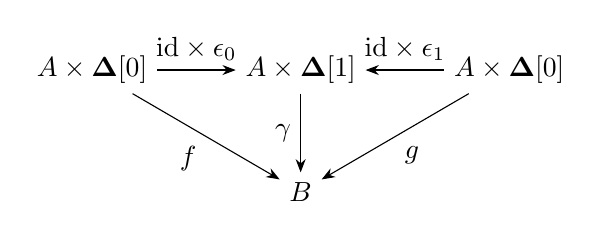
\begin{tikzpicture}[>=Stealth]
  % Nodes
	\node (A) {$A \times \D[1]$};
	\node[left=of A] (D) {$A \times \D[0]$};
	\node[right=of A] (B) {$A \times \D[0]$};
	\node[below=of A] (C) {$B$};

  % Arrows (legs of the right triangle)
	\draw[<-] (A) -- node[above] {$\text{id} \times \epsilon_1$} (B);
	\draw[->] (D) -- node[above] {$\text{id} \times \epsilon_0$} (A);
	\draw[<-] (C) -- node[below right] {$g$} (B);
	\draw[->] (D) -- node[below left] {$f$} (C);
    \draw[->] (A) -- node[left] {$\gamma$} (C);
\end{tikzpicture}
\caption{Simplicial Homotopy Diagram}
\label{simplicial-homotopy-diagram}
\end{figure}

Where $\text{id} \times \epsilon: A \times \D[0]$ is defined as $(a, \alpha) \mapsto (A, \epsilon_0 \circ \alpha)$, for $\alpha: [n] \to [0]$ in $\D$.

Notice that $\D[1]_n = \H([n], [1])$ has exactly $n + 2$ elements, corresponding to the $n + 2$ surjective maps from $[n]$ to $[1]$. 
Label them as $\alpha_i, -1 \leq i \leq n$.
So for each $n$, the map $ \gamma: A\times \D[1] \rightarrow B$ is determined by $n+2$ maps $\gamma^n_i: A_n \rightarrow B_n$ each corresponding to $\alpha_i \in \D[1]_n$.
For a temporary measure we call $\gamma$ as the middle map.

The following lemma is evident 

\begin{lemma}\label{homotopy-relation}
	Let $f, f', g, g', h$ be simplicial maps from $A$ to $B$, where $A$ $B$ are simplicial objects in abelian category $\A$. We have
	\begin{enumerate}
		\item $f \simeq f$
		\item If $f \simeq f'$ and $g \simeq g'$, then $f + g \simeq f' + g'$
		\item If $f \simeq f'$, then $(-f) \simeq (-f')$, $f-g \simeq 0$ and $g \simeq f$
		\item If $f \simeq g$ and $g\simeq h$, then $f \simeq h$
	\end{enumerate} 
\end{lemma}

\begin{proof}
	$f \simeq f$, as we can define $\gamma_i = f$ for all applicable $i$ in the commutative diagram \ref{simplicial-homotopy-diagram}.

	If $f\simeq g$ with corresponding $\gamma$ as middle maps and $f' \simeq g'$ with corresponding $\gamma'$ as middle maps, then $f + f' \simeq g + g'$ with corresponding $\gamma + \gamma'$ as the middle map.

	All other parts of the proof are similar.
\end{proof}

Here is an important lemma 

\begin{lemma}\label{homotopy-chain-homotopy1}
	If $f, g: A \rightarrow B$ are simplicial homotopic, then the induced map $f_{*}, g_{*}$ of normalised chain complexes $N(f), N(g): N(A) \rightarrow N(B)$ are chain homotopic.
\end{lemma}

\begin{proof}
	By lemma \ref{homotopy-relation}, $f \simeq g \iff f-g \simeq 0$. 
	So it suffices to show that if $f \simeq 0$, then $f_* = N(f) \simeq 0$ as chain maps.

	For each $n$, define $s_n = \sum_{i=0}^{n} (-1)^i h_i$, where $h_i$ are the maps in definition \ref{simplicial-homotopy} corresponding to the simplicial homotopy from $0$ to $f$.
	Note that $s_n$ is a map from $A_n$ to $B_{n + 1}$. 
	I claim that 
	\begin{equation}\label{chain-homotopy-eq}
		\d_{n+1} s_n - s_{n-1} \d_n = (-1)^n f
	\end{equation}
	, therefore $\{(-1)^n s_n\}$ is a chain homotopy from $0$ to $f_*$.
\begin{equation*}
	\begin{tikzcd}
		\cdots \arrow{r} & 
		N_n(A) \arrow{r}{\d_n} \arrow{d}{f_n} &
		\cdots \arrow{r}{\d_2} &
		N_1(A) \arrow{r}{\d_1} \arrow{d}{f_1} \arrow{dl}{s_1}&
		N_0(A) \arrow{r} \arrow{d}{f_0} \arrow{dl}{s_0}&
		0 \\
		\cdots \arrow{r} &
		N_n(B) \arrow{r}{\d_n} &
		\cdots \arrow{r}{\d_2} &
		N_1(B) \arrow{r}{\d_1} &
		N_0(B) \arrow{r} &
		0
	\end{tikzcd}
\end{equation*}
	Equation \eqref{chain-homotopy-eq} can be proved purely combinatorially.
	For the case $n = 0$, $s_0 = h_0$, and $d_1h_0$ by equation \eqref{homotopy1} is $f$.

	For the case $n = 1$, $s_1 = h_0 - h_1$.
	Therefore
	\begin{dmath}
		\d_{2}s_1 - s_0 \d_1 = \d_2 h_0 - \d_2 h_1 - h_0 \d_1
		= h_0 \d_1 - h_0 \d_1 - \d_2 h_1 \quad \text{by equation \eqref{homotopy2}}
		= -f \quad \text{by equation \eqref{homotopy1}}
	\end{dmath}

	All other cases can be proved similarly by expanding the left hand side of equation \eqref{chain-homotopy-eq} and applying equations \eqref{homotopy1} - \eqref{homotopy4} repeatedly to cancel out terms.
\end{proof}

There is a converse to lemma \ref{homotopy-chain-homotopy1}. 

\begin{lemma}\label{homotopy-chain-homotopy2}
	For two chain homotopic maps $f, g: C \rightarrow C'$, the corresponding simplicial maps $K(f), K(g): K(C) \rightarrow K(C')$ are simplicially homotopic.
\end{lemma}

\begin{proof}
	Assuming we have the chain homotopy $s_n: C_n \rightarrow C'_{n+1}$ from $f$ to $g$. 
	We shall define $h_i: K(C)_n \rightarrow K(C''_{n+1})$ according to the following procedure. 
	\begin{enumerate}
		\item On the unique summand $C_n$ of $K_n(C)$ corresponding to the identity map $\text{id}_{[n]}: [n] \to [n]$, define
		\begin{equation}
			h_i|_{C_n} = \begin{cases}
				\sigma_i f & i < n - 1 \\
				\sigma_{n - 1} f - \sigma_{n}s_{n-1}d & i = n - 1 \\
				\sigma_{n }( f - s_{n-1}d) - s_n & i = n - 1 \\
			\end{cases}
		\end{equation}
	\item On the summand $C_{n-1}[\eta]$ of $K(C)_n$ corresponding to a surjective map $\eta: [n] \to [n - 1]$. 
			Let $j$ be the integer such that $\eta_{j} = \eta_{j+1}$. 
			We can write $\eta =  \text{id}_{n-1} \circ \eta_j$, where $\eta_j$ is the $j$-th degenerate map in $\D$. 
			Note that $C_{n-1}[\text{id}_{n-1}]$ is isomorphic to $C_{n-1}[\eta_i]$.
			This is because we have the following commutative diagram 
\begin{equation*}
	\begin{tikzcd}
		{[n - 1]} \arrow{r}{\epsilon^i} \arrow{d}{\text{id}} & {[n]} \arrow{d}{\eta_i} \\
		{[n - 1]} \arrow{r}{\epsilon} & {[n - 1]}
	\end{tikzcd}
\end{equation*}
We have already defined the maps $h_i$ on $C_{n-1}[\text{id}_{n-1}]$, define $h'_i$ be the restriction of $h_i$ to $C_{n-1}[\text{id}_{n-1}]$. 
We define 
$$
h_i|_{C_{n-1}[\eta]} =
\begin{cases}
	\sigma_j h'_{i-1} & j < i\\'
	\sigma_{j+1} h'_{i} & j \geq i
\end{cases}
$$
\item On all other summands $C_p[\eta]$ of $K(C)_n$, with $\eta: [n] \rightarrow [p]$, find the greatest integer $j$ such that $\eta(j) = \eta(j + 1)$.
	We can write $\eta = \eta' \eta_j$,  and proceed similarly as in step 2.
	\end{enumerate}

	It is a lengthy but straightforward verification to check that the maps $h_i$ defined above satisfy equations \eqref{homotopy1} - \eqref{homotopy4} in definition \ref{simplicial-homotopy}.
\end{proof}


\section{Q4. Adjunction and Monads}

\subsection{Definitions of Monads and Adjunctions}

Let us first recall the definition of monads. 

\begin{definition}[Monad \cite{maclane}]
	A \emph{monad} (also called a triple) acting on a category $\C$ is a triple $(\top, \eta, \mu)$ where 
	\begin{itemize}
		\item $\top: \C \to \C$ is an endofunctor,
		\item $\eta: \text{id}_{\C} \Rightarrow \top$ is a natural transformation called the unit,
		\item $\mu: \top \circ \top \Rightarrow \top$ is a natural transformation called the multiplication.
	\end{itemize}
	such that we have the following three commutative diagrams.
	\begin{equation}\label{monad-associativity}
		\begin{tikzcd}
			\top\circ \top \circ \top (X) \arrow{r}{\top\mu_X} \arrow{d}{\mu_{\top X}} & \top \circ \top (X) \arrow{d}{\mu_X} \\
			\top \circ \top(X) \arrow{r}{\mu_X} & \top(X)
		\end{tikzcd}
	\end{equation}
	\begin{equation}\label{monad-unit}
		\begin{tikzcd}
			\top(X) \arrow{r}{\eta_{\top(X)}} \arrow{dr}{\text{id}_{\top(X)}} & \top \circ \top (X) \arrow{d}{\mu_X} \\
			 & \top(X)
		\end{tikzcd}, \quad
		\begin{tikzcd}
			\top(X) \arrow{r}{\top(\eta_X)} \arrow{dr}{\text{id}_{\top(X)}} & \top \circ \top (X) \arrow{d}{\mu_X} \\
			 & \top(X)
		\end{tikzcd}
	\end{equation}
	These three associtativity diagram can be summarised as the following identities for each object $X \in \C$, which will be crucial in the proof of construction of simplicial and cosimplicial objects from comonads and monads.
	\begin{align}
		\mu (\top \mu) =& \mu (\mu \top)\\ 
		\mu (\top \eta)=& \mu (\top \eta) = \text{id}
	\end{align}
\end{definition}

Also recall the definition of adjunction. 

\begin{definition}[Adjunction \cite{maclane}]
	An \emph{adjunction} between two categories $\A$ and $\B$ is a pair of functors $F: \A \rightleftarrows \B: G$ together with a natural isomorphism of hom-sets
	\begin{equation}
		\H_{\B}(F(X), Y) \cong \H_{\A}(X, G(Y))
	\end{equation}
	for all objects $X \in \A$ and $Y \in \B$. 
	In this case, we say that $F$ is left adjoint to $G$, and $G$ is right adjoint to $F$, denoted as $F \dashv G$.
\end{definition}

For a morphism $f: F(X) \rightarrow Y$, we shall denote its corresponding morphism under the natural isomorphism as $\overline{f}: X \rightarrow G(Y)$. 
The naturality condition can be summarised as 
\begin{equation}
\overline{F(X) \xrightarrow{f} Y \xrightarrow{g} Y'} =  X \xrightarrow{\overline{f}} G(Y) \xrightarrow{G(g)} G(Y')
\end{equation}
and 
\begin{equation}
\overline{X' \xrightarrow{f} X \xrightarrow{g} G(Y)} = F(X') \xrightarrow{F(f)} F(X) \xrightarrow{\overline{g}} Y
\end{equation}
For each $X \in A$, define $\eta_X = \overline{F(X) \xrightarrow{\text{id}} F(X)}$, which is a morphism from $X$ to $GF(X)$.
Similarly, for each $Y \in B$, define $\epsilon_Y = \overline{G(Y) \xrightarrow{\text{id}} G(Y)}$, which is a morphism from $FG(Y)$ to $Y$.

We have the following standard results from category theory.

\begin{lemma}\label{Unit-Counit}
	$\eta: \text{id}_{\A} \Rightarrow GF$ and $\epsilon: FG \Rightarrow \text{id}_{\B}$ are natural transformations called the unit and counit of the adjunction.
	Their commutative diagrams for naturality are as follows, where $X, X' \in \A, Y, Y' \in \B, f: A \rightarrow A'$ and $g: B \rightarrow B'$, 
	\begin{equation}
		\begin{tikzcd}
			X \arrow{r}{f} \arrow{d}{\eta_{X}} &  X' \arrow{d}{\eta_{X'}} \\
			GF(X) \arrow{r}{f} & GF(X')
		\end{tikzcd}
		\quad
		\begin{tikzcd}
			F G (Y) \arrow{r}{FG g} \arrow{d}{\epsilon_{FG(Y)}} &  FG (Y') \arrow{d}{\epsilon_Y} \\
			Y \arrow{r}{g} & Y'
		\end{tikzcd}
	\end{equation}
\end{lemma}

\begin{lemma}\label{commutative-units-counit}
	For $X \in \A$ and $Y \in \B$, the following two diagrams commute.
	\begin{equation}\label{adj-triangle}
		\begin{tikzcd}
			F(X) \arrow{r}{F(\eta_X)} \arrow{dr}{\text{id}_{F(X)}} & FGF(X) \arrow{d}{\epsilon_{F(X)}} \\
			 & F(X)
		\end{tikzcd}
		\quad
		\begin{tikzcd}
			G(Y) \arrow{r}{\eta_{G(Y)}} \arrow{dr}{\text{id}_{G(Y)}} & GFG(Y) \arrow{d}{G(\epsilon_{Y})} \\
			 & G(Y)
		\end{tikzcd}
	\end{equation}
\end{lemma}

\subsection{Monads from Adjunctions}

We can construct a monad from an adjunction as follows.

\begin{theorem}
	Let $F: \A \rightleftarrows \B: G$ be an adjunction with unit $\eta$ and counit $\epsilon$. 
	Define $\top = G\circ F$. 
	Unit of $\top$ is given by the unit of adjunction $\eta: \text{id}_{\A} \to G \circ F$. 
	Multiplication is induced by the counit 
	$$
		\mu : \top \circ \top = GFGF \xrightarrow{G \epsilon F} GF = \top.
	$$
	Then $(\top, \eta, \mu)$ is a monad acting on the category $\A$.
\end{theorem}

\begin{proof}
	We need to check the three conditions of monads separately.

	First consider the diagram
	\begin{equation}
		\begin{tikzcd}
			F G F G  (Y) \arrow{r}{FG \epsilon_x} \arrow{d}{\epsilon_{FG(Y)}} &  FG (Y) \arrow{d}{\epsilon_Y} \\
			F G (Y) \arrow{r}{\epsilon_X} & Y
		\end{tikzcd}
	\end{equation}
	Notice this is exactly the diagram for naturality of $\epsilon$ shown in lemma \ref{Unit-Counit}, with $Y = FG(Y)$, $Y' = Y$.
	Left compose this diagram with $G$ and right compose with $F$, we have the following commutative diagram
	\begin{equation}
		\begin{tikzcd}
			G F G F G F (Y) \arrow{r}{GFG\epsilon_{F(Y)}} \arrow{d}{G \epsilon_{FGF(Y)}} &  G F G F(Y) \arrow{d}{G \epsilon_{F(X)}} \\
			G F G F(Y) \arrow{r}{G\epsilon_{F(Y)}} & G F(Y)
		\end{tikzcd}
	\end{equation}
	This is exactly the associativity diagram \eqref{monad-associativity} for the monad $(\top, \eta, \mu)$.

	By lemma \ref{commutative-units-counit} we have the following two commutative diagrams.
	$$
		\begin{tikzcd}
			F(X) \arrow{r}{F(\eta_X)} \arrow{dr}{\text{id}_{F(X)}} & FGF(X) \arrow{d}{\epsilon_{F(X)}} \\
			 & F(X)
		\end{tikzcd}
		\quad
		\begin{tikzcd}
			G(Y) \arrow{r}{\eta_{G(Y)}} \arrow{dr}{\text{id}_{G(Y)}} & GFG(Y) \arrow{d}{G(\epsilon_{Y})} \\
			 & G(Y)
		\end{tikzcd}
	$$
	Precompose the left diagram with $G$ and postcompose with $F$ gives us 
	$$
		\begin{tikzcd}
			GF(X) \arrow{r}{GF(\eta_X)} \arrow{dr}{\text{id}_{GF(X)}} & GFGF(X) \arrow{d}{G\epsilon_{F(X)}} \\
			 & GF(X)
		\end{tikzcd}
		\quad
		\begin{tikzcd}
			G F (Y) \arrow{r}{\eta_{GF(Y)}} \arrow{dr}{\text{id}_{G(Y)}} & GFGF(Y) \arrow{d}{G\epsilon_{F(Y)}} \\
			 & G(Y)
		\end{tikzcd}
	$$
	Which is exactly the two diagrams in \eqref{monad-unit} for the monad $(\top, \eta, \mu)$.
	Hence we have verified all the conditions for $(\top, \eta, \mu)$ and conclude that it is indeed a monad acting on the category $\A$.

\end{proof}

\subsection{Comonads from Adjunctions}

The definition of Comonads is dual to that of monad by reversing all the arrows. 
The preciese definition is listed below.
 
\begin{definition}[Comonad \cite{maclane}]
	A \emph{comonad}, also called \emph{cotriple}, acting on a category $\C$ is a triple $(\perp, \epsilon, \delta)$ where 
	\begin{itemize}
		\item $\perp: \C \to \C$ is an endofunctor,
		\item $\epsilon: \perp \Rightarrow \text{id}_{\C}$ is a natural transformation called the counit,
		\item $\delta: \perp \Rightarrow \perp \circ \perp$ is a natural transformation called the comultiplication.
	\end{itemize}
	such that we have the following three commutative diagrams.
	\begin{equation}\label{comonad-coassociativity}
		\begin{tikzcd}
			\perp (X) \arrow{r}{\delta_{X}} \arrow{d}{\delta_{X}} & \perp \circ \perp (X) \arrow{d}{\perp \delta_X} \\
			\perp \circ \perp(X) \arrow{r}{\delta_{\perp X}} & \perp \circ \perp \circ \perp(X)
		\end{tikzcd}
	\end{equation}
	\begin{equation}\label{comonad-counit}
		\begin{tikzcd}
			\perp(X) \arrow{r}{\delta_{X}} \arrow{dr}{\text{id}} & \perp \circ \perp (X) \arrow{d}{\epsilon_{\perp(X)}} \\
			 & \perp(X)
		\end{tikzcd}, \quad
		\begin{tikzcd}
			\perp(X) \arrow{r}{\delta_{X}} \arrow{dr}{\text{id}} & \perp \circ \perp (X) \arrow{d}{\perp\epsilon_{X}} \\
			 & \perp(X)
		\end{tikzcd}
	\end{equation}
	These three coassocitativity diagram can be summarised as the following identities for each object $X \in \C$, which will be crucial in the proof of construction of simplicial and cosimplicial objects from comonads and monads.
	\begin{align}
		(\perp \delta) \delta =& (\delta \perp) \delta \label{comonad-asso} \\ 
		(\epsilon \perp)=& (\perp \epsilon) = \text{id} \label{comonad-counit-id}
	\end{align}
\end{definition}

We may construct a comonad from an adjunction as follows.

\begin{theorem}
	Let $F: \A \rightleftarrows \B: G$ be an adjunction with unit $\eta$ and counit $\epsilon$. 
	Define $\perp = F\circ G$. 
	Counit of $\perp$ is given by the counit of adjunction $\epsilon: F \circ G \to \text{id}_{\B}$. 
	Comultiplication is induced by the unit 
	$$
		\delta : \perp = F G \xrightarrow{F \eta G} F G F G = \perp \circ \perp.
	$$
	Then $(\perp, \epsilon, \delta)$ is a comonad acting on the category $\B$.
\end{theorem}

The proof is exactly dual to that of monads from adjunctions, by reversing all the arrows, and is therefore omitted here.

Here is an important observation.

\begin{remark}
	A monad on $\A$ is the same as a comonad on the opposite category $\A^{op}$.
\end{remark}

\section{Simplical Objects and Monads}

A comonad may induce a simplicial object.

\begin{theorem}
	Let $(\perp, \epsilon, \delta)$ be a comonad acting on a category $\A$.
	Define a simplicial object $\perp_{\bullet}$ in $\A$ as follows.
	\begin{itemize}
		\item For each $n \geq 0$, define $\perp_n := \perp[n] = \perp^{n+1} A$. Here $\perp^{n+1}$ means compostion of $\perp$ with itself $n+1$ times.

		\item For each $n \geq 1$ and $0 \leq i \leq n$, define the face maps $\d_i^n: \perp_n \to \perp_{n-1}$ as
		\begin{equation}
			\d_i^n = \perp^i \epsilon \perp^{n-i} \quad : \quad \perp^{n+1} A \to \perp^n A
		\end{equation}

		\item For each $n \geq 0$ and $0 \leq i \leq n$, define the degeneracy maps $\sigma_i^n: \perp_n \to \perp_{n+1}$ as
		\begin{equation}
			\sigma_i^n = \perp^i \delta \perp^{n-i}\quad : \quad \perp^{n+1} A \to \perp^{n+2} A
		\end{equation}
	\end{itemize}
	Then $(\perp_{\bullet}, \d_i, \sigma_i)$ is a simplicial object in the category $\A$.
\end{theorem}
As usually, the domain and the range of the face and degeneracy maps will always be evident from the context, and the superscript will therefore be omitted.

\begin{proof}
	We will verify $\perp_\bullet$ is indeed a monad following the remark \ref{sim-set-data}; i.e., the faces and degeneracy map satisfy the simplicial identities listed in \eqref{simp1} to \eqref{simp3}.

	We shall first of all unpack the notation. 
	\begin{align*}
		\d_i \sigma_i   =& \perp^i(\epsilon \perp) \delta \perp^{n-i} \\ 
						=& \perp^i (\text{id}) \perp^{n-i} \quad \text{by \eqref{comonad-asso}} \\	
						=& \text{id} 
	\end{align*}

	Similarly, 
	\begin{align*}
		\d_{i+1} \sigma_i =& \perp^i(\perp \epsilon) \delta \perp^{n-i} \\ 
						=& \perp^i (\text{id}) \perp^{n-i} \quad \text{by \eqref{comonad-counit-id}} \\	
						=& \text{id} 
	\end{align*}

	All the rest of the identities can be verified in a similar manner by applying \eqref{comonad-asso} and \eqref{comonad-counit-id} at the appropriate places.
\end{proof}

Dually, a monad may induce a cosimplicial object. 

\begin{theorem}
	Let $(\top, \eta, \mu)$ be a monad acting on a category $\A$.
	Define a cosimplicial object $L^{\bullet}$ in $\A$ as follows.
	\begin{itemize}
		\item For each $n \geq 0$, define $L^n := \top^{n+1} A$. Here $\top^{n+1}$ means compostion of $\top$ with itself $n+1$ times.

		\item For each $n \geq 0$ and $0 \leq i \leq n$, define the coface maps $\d^i_n: \top^n \to \top^{n+1}$ as
		\begin{equation}
			\d^i_n = \top^i \eta \top^{n-i} \quad : \quad \top^{n+1} A \to \top^{n+2} A
		\end{equation}

		\item For each $n \geq 1$ and $0 \leq i \leq n-1$, define the codegeneracy maps $\sigma^i_n: \top^n \to \top^{n-1}$ as
		\begin{equation}
			\sigma^i_n = \top^i \mu \top^{n-i}\quad : \quad \top^{n+1} A \to \top^{n} A
		\end{equation}
	\end{itemize}
	Then $(\top^{\bullet}, \d^i, \sigma^i)$ is a cosimplicial object in the category $\A$.
\end{theorem}

The proof is exactly identity to that of simplicial objects from comonads, by reversing all the arrows, and is therefore omitted here.


\section{Q6. Canonical Resolutions}

This section aims to solve the following problem.

\begin{problem}
	Let $R$ be a ring and $(F, U)$ the free-forgetful adjunction between the category between $\RM$ and $\S$.
	$\perp := FU$, therefore, is a comonad on $\RM$. 
	Pick an $M\in \RM$, we can construct a simplicial set $\perp^\bullet M$.
	Let $N$ be a right $R$-module, and define $E$ as $-\otimes_{R}$. Therefore $E(\perp^\bullet M)$ is a also an simplicial object.

	Recall Dold-Kan correspondence that an simplicial object induces a normalised chain complex via the functor $N$.
	Define $H_n(M, E)$ as the $n$-th homology of the normalised chain complex $N(E(\perp^\bullet M))$.
	Prove that 
	\begin{equation}\label{p6}
		H_n(M, E) \cong \T^R_n(M, N)
	\end{equation}
\end{problem}

The key to solve this problem is the fact that the chain complex $N(\perp^\bullet M)$ is a free resolution of $M$. 
Therefore \eqref{p6} follows from the definition of Tor-functor.

Recall each term in $N(\perp^\bullet M)$ is given by
\[
	N(\perp^\bullet M)_n = \bigcap_{i=1}^n \ker(d_i) \subset \perp^{n+1} M = (FU)^{n+1} M
\]
Since $F$ is free functor, each term in the chain complex is a free $R$-module.
So the only obstacle is to show the chain complex is exact.
\begin{theorem}\label{canonical-resolution-exact}
	For any $M \in \RM$, the normalised chain complex $N(\perp^\bullet M)$ is exact. 
\end{theorem}

This theorem is can be proved in several steps via the method in contractible simplicial objects.

\begin{definition}[Contractible]
	A simplicial object $X$ is \emph{contractible} if there exists maps $s_{f}: X_n \to X_{n+1}$ for each $n\geq 0$ such that
	\begin{align}
		\d_{n+1}f_{n} &= \id \label{contractible1} \\
		\d_{i}f_{n} &= f_{n-1}\d_{i} \quad \text{for } 0 \leq i \leq n \label{contractible2} 
	\end{align}
\end{definition}

The following lemma is evident.

\begin{lemma}\label{contractible-exact}
	If $X$ is a contractible simplicial object, then the associated normalised chain complex $N(X)$ is exact.
\end{lemma}

\begin{proof}
	Let $X$ be a contractible simplicial object with contracting homotopies $f_n: X_n \to X_{n+1}$.
	The associated normalised chain complex $N(X)$ has differential $d_n = \d_n|_{N(X)_n}$.
	
	Combining these we have the following diagram.
	\begin{equation*}
	\begin{tikzcd}
		\cdots \arrow{r} & 
		N_{n+1}(X) \arrow{r}{\d_{n+1}}&
		N_n(X) \arrow{r}{\d_n} \arrow[shift left]{l}{f_n}&
		N_{n-1}(X) \arrow{r}       \arrow[shift left]{l}{f_{n-1}}&
		\cdots 
	\end{tikzcd}
	\end{equation*}
	Here, we have use some abuse of notation as $\im{f_n}$ may not lie in $N_{n+1}(X)$. 

	Assuming $x \in N_n(X)$ with $\d_n x = 0$. 
	Since $N_n(X) = \bigcap_{i=0}^{n-1}\ker \d_i$, we conclude $\d_i x = 0$ for all $0 \leq i \leq n$. 
	By \eqref{contractible2}, we have $\d_i f_n(x) = f_{n-1} \d_i x = 0$ for all $0 \leq i \leq n$, that is $f_n(x) \in N_{n+1}(X)$.
	Again, applying \eqref{contractible1}, we have $\d_{n+1} f_n(x) = x$, so $x \in \im{\d_{n+1}}$.

	This shows that $\ker{\d_n} \subset \im{\d_{n+1}}$.
	Therefore the chain complex $N(X)$ is exact.
\end{proof}

The following lemma is also crucial.
\begin{lemma}\label{adjoint-contractible}
	Suppose that $U: \A \rightarrow \B$ has a left adjoint $F: \B \rightarrow \A$.
	Then for any $A \in \A$, the simplicial object $U(\perp_\bullet A)$ is contractible.
\end{lemma}

\begin{proof}
	Define $f_n = \eta U\perp^n$, we can see all the required conditions hold.
\end{proof}

From now the argument is easy.
Using the notation of lemma \ref{adjoint-contractible}, let $\A = \RM$, $\B = \S$ and $A = M$. 
Therefore $U(\perp_\bullet M)$ is a contractible simplicial set.
Since forgetful functor does not change the mapping or the underlying set structure, but only forgets the module structure, therefore $\perp_\bullet M$ is also contractible as a simplicial set.
Therefore, applying lemma \ref{contractible-exact}, the normalised chain complex $N(\perp^\bullet M)$ is exact, which completes the proof for theorem \ref{canonical-resolution-exact}.

\section{Q7. Relative Homology and Hochschild Homology}

Given a ring homomorphism $f: R \to k$, there is a forgetful functor $U: \MR \to \Mk$.
It has a left adjoint $F: \Mk \to \MR$ defined by $F(M) = M \otimes_k R$.
Therefore $(F, U)$ constittutes a comonad $\perp = FU$ on $\MR$, and thus we can construct a simplicial object $\perp_\bullet M$ for any $M \in \MR$.

By definition of $(F, U)$, it is evident that $\perp M = M \otimes_k R$, and thus $\perp_n = \perp^{n+1} M = M \otimes_k R^{\otimes n}$.
Note that Lemma \ref{adjoint-contractible} still holds in this case, so the normalised chain complex $N(\perp_\bullet M)$ is exact considered as complex of $k$-modules.

Based on this observation, we define Bar resolution as follows.

The relative $\T$ group $\T^{R/k}(M, N)$ is defined as the homology of the normalised chain complex $N(\perp_\bullet M \otimes_R N)$.
Similarly, the relative $\E$ group $\E_{R/k}^n(M, N)$ is defined as the cohomology of the normalised cochain complex $N(\H_R(\perp_\bullet M, N))$.

\begin{definition}[Bar Resolution] 
	Given a ring homomorphism $k \to R$ and an $R$-module $M$, and its associated comonad $\perp = FU$ on $\MR$ as defined above,
	the \emph{Bar resolution} of $M$ over $k$ is the unnormalised chain complex a $\perp_\bullet M$ considered as a chain complex of $k$-modules.

	Precisely, each term in the Bar resolution is given by 
	\[
		\beta_n(R, M) = \perp_n M = M \otimes_k R^{\otimes (n+1)}
	\]
\end{definition}

We are now ready to define Hochschild homology and cohomology.
\begin{definition}[Hochschild Homology and Cohomology]
	Let $k$, $R$ be rings with a ring homomorphism $k \to R$. 
	Then we have the free-forgetful adjunction $(F, U)$ between $\MR$ and $\Mk$ as above, and a comonad $\perp = FU$ on $\MR$.

	Define $R^e$ as the enveloping algebra $R \otimes_k R^{op}$.
	The \emph{Hochschild homology} $HH_n(R, M)$ is defined as the relative $\T$ group $\T^{R/k}_n(R^e, N)$.
	The \emph{Hochschild cohomology} $HH^n(R, M)$ is defined as the relative $\E$ group $\E_{R/k}^n(R^e, N)$.
\end{definition}

We want to solve the following problem. 
\begin{problem}
	If $R$ is flat as a $k$-module prove that 
	$$
	HH_n(R, N) \cong \T_n^{R^e}(R, N)
	$$
	where the right hand side is the usual Tor-functor over the ring $R^e$.
	If $R$ is projective as a $k$-module prove that 
	$$
	HH^n(R, N) \cong \E^n_{R^e}(R, N)
	$$
	where the right hand side is the usual Ext-functor over the ring $R^e$.
\end{problem}

\begin{proof}
	If each $R$ is flat as a $k$-module, then every $R^{\otimes n}$ is also a flat $k$ module, as tensor product preserves flatness.
	Therefore each term in the Bar resolution $\beta_n(R, R) = R^e \otimes_k R^{\otimes n}$ is also flat as an $R^e$-module by the change of ring flatness property.
	Therefore the Bar resolution is a flat resolution of $R^e$ as an $R^e$-module, and $HH^n(R, N)$ computes the $n$-th homology group of the complex $\beta_\bullet(R, R^e) \otimes_{R} N$, which is the same as $\T_n^{R^e}(R, N)$.

	One caveat is that $\T$ is usually defined via projective resolutions, but here we have flat resolution. 
	This creates no problem since derived functors forms a universal $\delta$-functor, and computation via flat resolutions will gives the same result.

	The proof for cohomology case is exactly the same by replacing flat modules with projective modules, and tensor product with Hom-functor.
\end{proof}

\section{Further Discussion}

This section provides some further discussion on the relation between Hochschild homology and Kahler differentials, and introduces Andre-Quillen cohomology.
Most of the content here is based on \cite{weibel}.

Let us first define Kahler differentials. 

\begin{definition}[Kahler Differentials]
	Let $k \to R$ be a ring homomorphism.
	The module of \emph{Kahler differentials} $\Omega_{R/k}$ is defined as the $R$-module generated by symbols $d r$ for each $r \in R$, subject to the following relations:
	\begin{align*}
		d(r_1 + r_2) &= dr_1 + dr_2 \\
		d(r_1 r_2) &= r_1 dr_2 + r_2 dr_1 \\
		d(k) &= 0 \quad \text{for all } k \in k
	\end{align*}
\end{definition}

If $M$ is a $k$-derivation is a $k-$module homomorphism $D: R \to M$ such that $D(r_1 r_2) = r_1 D(r_2) + r_2 D(r_1)$ for all $r_1, r_2 \in R$.
The map $d: R \to \Omega_{R/k}$ defined by $r \mapsto dr$ is a $k$-derivation.
Denote the set of all $k$-derivations from $R$ to $M$ as $\text{Der}_k(R, M)$. 
It is an $R$ module via $(rD)(r') = r D(r')$ for all $r, r' \in R$ and $D \in \text{Der}_k(R, M)$.


We have the following universal property. 
\begin{theorem}[Universal Property of Kahler Differentials]
	For any $R$-module $M$, there is a natural isomorphism
	\[
		\H_R(\Omega_{R/k}, M) \cong \text{Der}_k(R, M)
	\]
\end{theorem}

\subsection{HKR Theorem} 

We have the following statement at degree one. 

\begin{theorem}
For a $k$-algebra $R$, its module of Kahler differentials $\Omega_{R/k}$ is isomorphic to the first Hochschild homology $HH_1(R, R)$.
\end{theorem}

For degree greater than one, define degree-$n$ Kahler forms as follows.
\begin{definition}[Kahler n-forms]
	Let $k \to R$ be a ring homomorphism.
	The module of \emph{Kahler n-forms} $\Omega^n_{R/k}$ is defined as the $n$-th exterior power of $\Omega_{R/k}$:
	\[
		\Omega^n_{R/k} := \bigwedge^n_R \Omega_{R/k}
	\]
\end{definition}

By restricting to a well behaved class of rings, we have the following beautiful result connecting Hochschild homology and Kahler differentials.

\begin{theorem}[Hochschild-Kostant-Rosenberg theorem]
	If $k$ is a field and $A$ is a commutative $k$-algebra satisfying:
	\begin{enumerate}
		\item $A$ is finitely regenerated 
		\item The $A$ module of Kahler differentials $\Omega_{A/k}$ is projective
	\end{enumerate}
	Then there is an isomorphism of $A$-algebras 
	\[
		HH_n(A, A) \cong \Omega^n_{A/k}
	\]

	Dually, there is a isomorphism of Hochschild cohomology and wedge product of Kahler differentials:
	\[
		HH^n(A, A) \cong \bigwedge^n_A Der_k(A, A)
	\]
\end{theorem}

This theorem is proved by Weibel \cite{weibel} in Theorem 9.4.7.

\subsection{Andre-Quillen Cohomology}

We are now ready to state Andre-Quillen cohomology. 

\begin{definition}[Andre-Quillen Cohomology]
	Let $k \to R$ be a ring homomorphism, and $M$ an $R$-module.
	The \emph{Andre-Quillen cohomology} $D^n(R/k, M)$ with values in an $R-$module $M$ is a cotriple cohomology of $R$ wtih coefficients in $Der_k(-, M)$:
	\[
		D^n(R/k, M) := H^n(R; Der_k(-, M))
	\]
\end{definition}

Its relation to Hochschild theory is via the following theorm by Barr. 

\begin{theorem}[Barr]
	Suppose $C_\bullet(R)$ is an $R-$module chain complex, natural in $R$ for each commutative $k-$algebra $R$, such that 
	\begin{enumerate}
		\item $H_0(C_\bullet(R)) \cong \Omega(R/k)$ for all $R$
		\item If $R$ is a polynomial algebra over $k$, $C_\bullet(R) \rightarrow \Omega(R/k)$ is a split exact resolution 
		\item For each $p$ there is a functor $F_p: k-\textbf{mod} \rightarrow k-\textbf{mod}$ such that $C_p(R) \cong R\otimes_k F_p(UR)$, where $UR$ is the underlying $k-$module of $R$.
	\end{enumerate}
	Then there is a natural isomorphism 
	\[
		D^n(R/k, M) \cong H^n(\H_R(C_\bullet(R), M))
	\]
\end{theorem}


\newpage

\printbibliography[heading=bibintoc]

\end{document}
